\documentclass[t, aspectratio = 137, xcolor=dvipsnames,table,compress]{beamer}
\geometry{papersize={12cm,6.75cm}}
\usetheme{Luebeck}
%\usetheme{moloch}

\useoutertheme{infolines}


%\usepackage[cache=false]{minted} %the output dir made it display correctly. wild

\usepackage{pdfpages}

\usepackage{amsmath,graphicx}
\usepackage{eso-pic}

\usepackage{array}


\usepackage[english]{babel}
% or whatever

\usepackage[latin1]{inputenc}
% or whatever


\usepackage{ wasysym }

\usepackage{multicol}

%\usepackage{beramono}
\usepackage[ocr-b-outline]{ocr}
%\usepackage[T1]{fontenc}




\setbeamertemplate{footline}{% 
  \hfill% 
  \usebeamercolor[fg]{page number in head/foot}% 
  \usebeamerfont{page number in head/foot}% 
  \insertframenumber%
  %\,/\,\inserttotalframenumber
  \kern1em\vskip2pt% 
}

%\useoutertheme{infolines} %show single section/subsection at the top
\beamertemplatenavigationsymbolsempty % get rid of navigation bar
%\setbeamertemplate{footline}[frame number]{} % remove bottom bar (not page number though)

% %gets rid of bottom navigation bars
% \setbeamertemplate{footline}[frame number]{}

% %gets rid of bottom navigation symbols
% \setbeamertemplate{navigation symbols}{}

% %gets rid of footer
% %will override 'frame number' instruction above
% %comment out to revert to previous/default definitions
% \setbeamertemplate{footline}{}


\usepackage[absolute,overlay]{textpos}
\setlength{\TPHorizModule}{30mm}
\setlength{\TPVertModule}{\TPHorizModule}
\textblockorigin{10mm}{10mm} 

\setbeamertemplate{caption}{\raggedright\insertcaption\par} %no 'figure' in the caption
 
\usepackage{epsfig} 
\usepackage{footnpag} 
\def\thefootnote{\fnsymbol{footnote}}
\usepackage{graphicx,epstopdf}
\usepackage{xspace}
\usepackage{mathtools}
\usepackage{tikz}
\usepackage{xcolor}
\usepackage{pgffor}

\usepackage{MnSymbol,wasysym}
%\usepackage{emoji}


%allow tikz pictures

\usepackage{tikz}



%this makes \ell from l in math mode
\mathcode`l="8000
\begingroup
\makeatletter
\lccode`\~=`\l
\DeclareMathSymbol{\lsb@l}{\mathalpha}{letters}{`l}
\lowercase{\gdef~{\ifnum\the\mathgroup=\m@ne \ell \else \lsb@l \fi}}%
\endgroup


%% Don't use navigation symbols (Distracting)
\setbeamertemplate{navigation symbols}{}

\setbeamertemplate{items}[ball] 


\setbeamertemplate{page number in head/foot}{}



% %%%
% % SUBFIGURE
% %%%
\usepackage{graphicx}
\usepackage{subcaption} % For subfigure support


 %%% PUT TEXT AT BOTTOM OF SLIDE
%Reference: https://tex.stackexchange.com/questions/54180/how-do-i-write-something-at-the-end-of-the-slide-in-beamer
% Note: When using this command,  \vfill will not work as normally.  Instead you would have to manually choose a unit of measurement for the amount of blank space,  e.g. \vskip10ex (approximatley 10 times the height of an x in the current font), \vskip2in, or whatever.  See https://tex.stackexchange.com/questions/8260/what-are-the-various-units-ex-em-in-pt-bp-dd-pc-expressed-in-mm for more on measurements.
\newcommand{\citebottom}[1]{
\vskip0pt plus 1filll  \tiny {#1}
}



\begin{document}

\newtheorem{thm}{Theorem}[section]
\newtheorem{cor}[thm]{Corollary}
\newtheorem{lem}[thm]{Lemma}
\newtheorem{prop}[thm]{Proposition}
\newtheorem{claim}[thm]{Claim}
\newtheorem{remark}[thm]{Remark}
\newtheorem{conj}[thm]{Conjecture}
\newtheorem{quest}[thm]{Question}
\newtheorem{prob}[thm]{Problem}
\newtheorem{obs}[thm]{Observation}
\newtheorem{ex}[thm]{Example}
\newtheorem{axiom}[thm]{Axiom}
\newtheorem{alg}[thm]{Algorithm}

\AtBeginEnvironment{defi}{%
  \setbeamercolor{block title}{use=example text,fg=white,bg=example text.fg!75!black}
  \setbeamercolor{block body}{parent=normal text,use=block title example,bg=block title example.bg!10!bg}
}

\newcommand{\cp}[1]{{\color{red}{Cory: #1}}}


\theoremstyle{definition}
\newtheorem{defi}{Definition}





%%%%%%%%%
%% Colors
%%%%%%%%%
%% \def\hicoli{\OliveGreen}
%% \def\hicoliv{\Magenta}
\newcommand{\hicoli}[1]{{\color{OliveGreen}{#1}}}
\newcommand{\hicolv}[1]{{\color{Magenta}{#1}}}
%% \newcommand{\hicolii}[1]{{\color{Maroon}{#1}}}
\newcommand{\hicolii}[1]{{\color{red!45!black}{#1}}}
\newcommand{\redbrightcol}[1]{{\color{red!75!black}{#1}}}
%% U de M version
%% \newcommand{\hicoliii}[1]{{\color{blue!40!black}{#1}}}
\newcommand{\hicoliii}[1]{{\color{blue!65!black}{#1}}}
\newcommand{\hicoliv}[1]{{\color{green!45!black}{#1}}}
\newcommand{\defcol}[1]{{\color{OliveGreen}{#1}}}
\newcommand{\origcol}[1]{{\color{Black}{#1}}}
\newcommand{\inviscol}[1]{{\color{White}{#1}}}

\newcommand{\graycol}[1]{{\color{white!50!black}{#1}}}


 \newcommand\soln[1]{{\color{orange}\small \noindent\textsc{Solution:}\noindent{ #1}}}
 



%% \setbeamertemplate{title page} 
%% { 
%% \begin{centering} 
%% {\usebeamerfont{title}\usebeamercolor[fg]{title}\inserttitle} 
%% \insertdate 
%% \end{centering} 
%% } 









\title{CSCI 246 -- Discrete Structures} 
\author{Mike Wojnowicz}

\institute{Montana State University}

\date{Spring 2025}{}



%\begin{frame}[plain, noframenumbering]
%\begin{multicols}{2}
%  \tableofcontents
%\end{multicols}
%\end{frame}

\renewcommand{\insertframenumber}{}


\begin{frame}[plain,label=title-page, noframenumbering ]
  \titlepage
\end{frame}



\begin{frame}{CSCI 246 -- Discrete Structures}

 \begin{block}{Delayed start}
 
We will start at 2:15 today due to the last-minute room change.

\vspace{0.2cm}

Feel free to 
\begin{itemize}
\item Check out the syllabus ahead of time on Brightspace
\item Meet a neighbor
\item Meditate
\item Brag to your friends about how much you're going to learn about discrete structures!	
\item [...]
\end{itemize}

\end{block}
	
\end{frame}


\begin{frame}{Syllabus Review}

\Large \centering
\vfill 
See Brightspace for syllabus.

\end{frame}


\begin{frame}{What is Discrete Math}
\begin{figure}
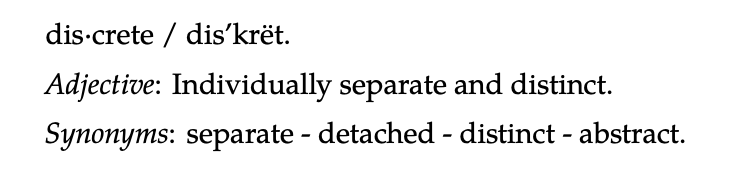
\includegraphics[width=0.9\textwidth]{images/what_is_discrete_math}
\end{figure}
\end{frame}


 
\begin{frame}{Why Active Learning?}


\begin{figure}[h!]
    \centering
    % Top row with two pictures
    \begin{subfigure}{0.45\textwidth}
        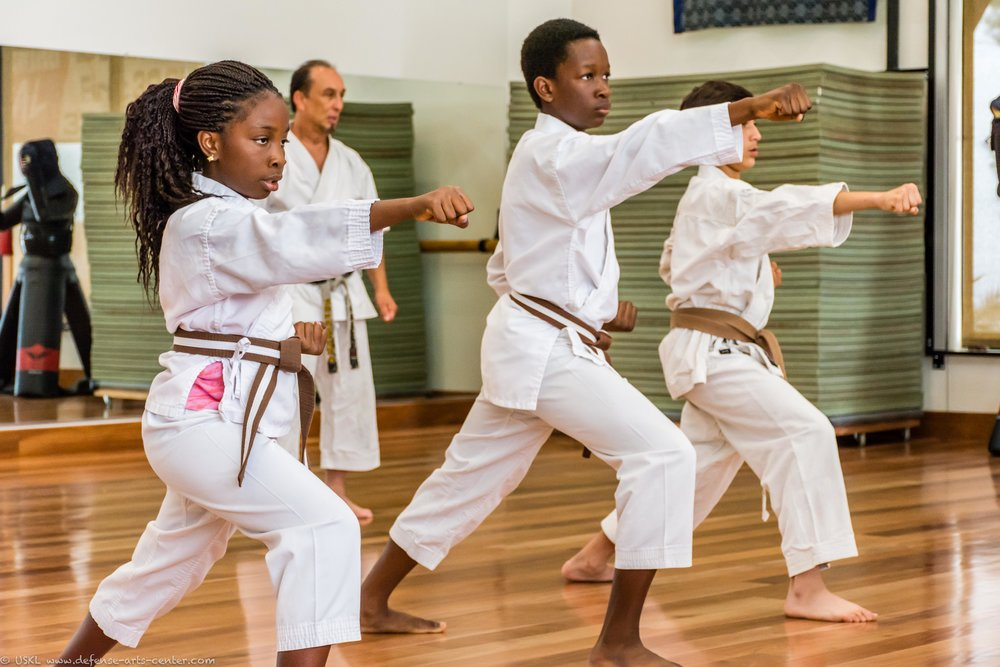
\includegraphics[width=0.8\textwidth]{images/karate} 
        %\caption{Picture 1}
    \end{subfigure}
    \hfill
    \begin{subfigure}{0.45\textwidth}
        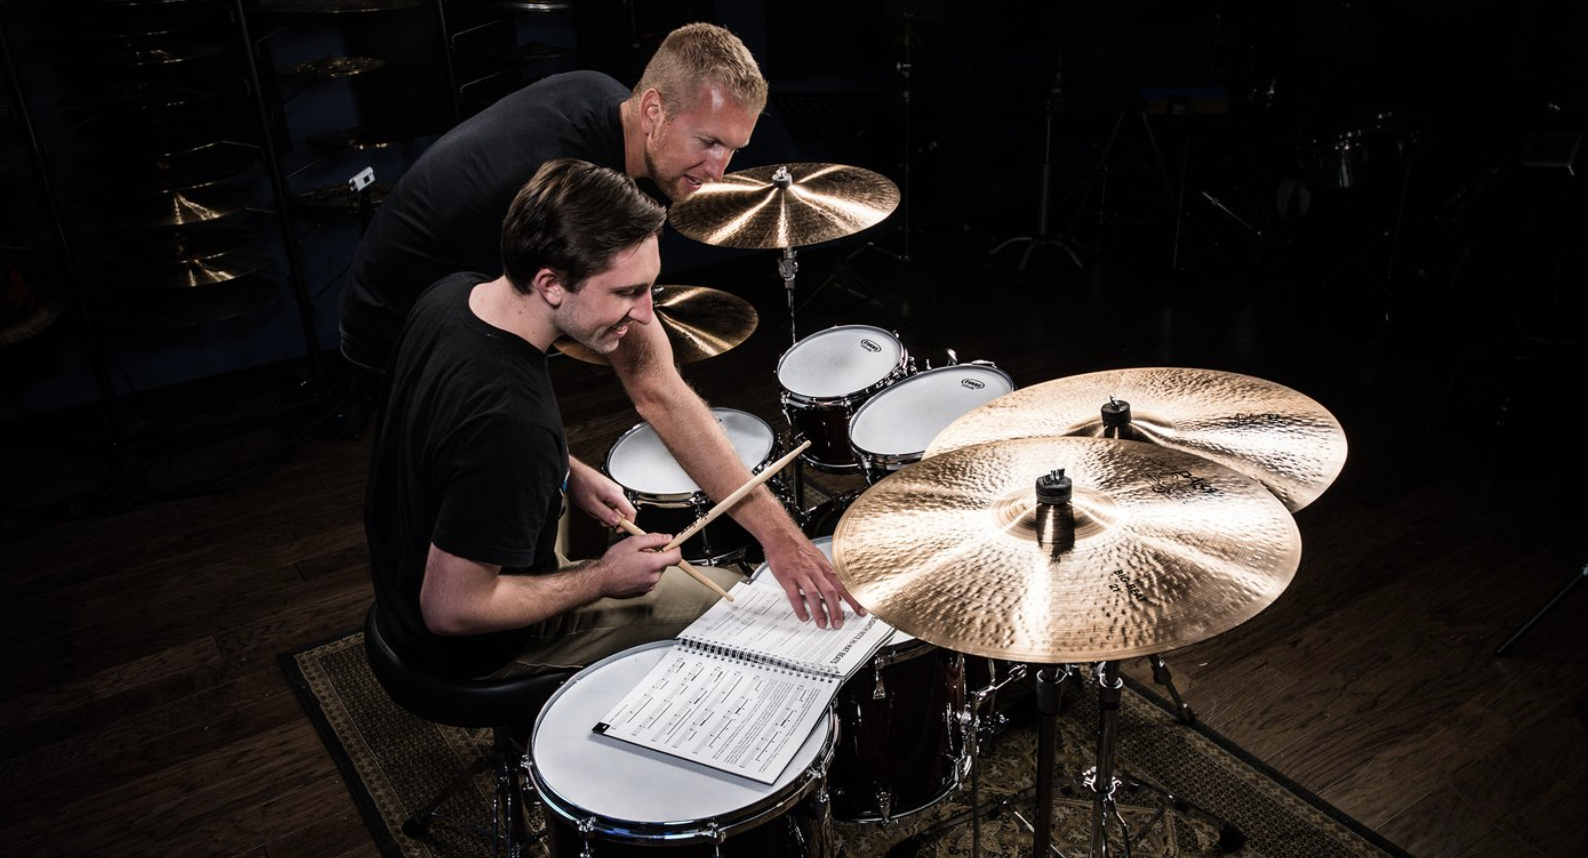
\includegraphics[width=0.8\textwidth]{images/drums} 
        %\caption{Picture 2}
    \end{subfigure}
    
    % Bottom row with one picture
    %\vspace{0.5em} % Add vertical space between rows
    \begin{subfigure}{0.5\textwidth}
        \centering
        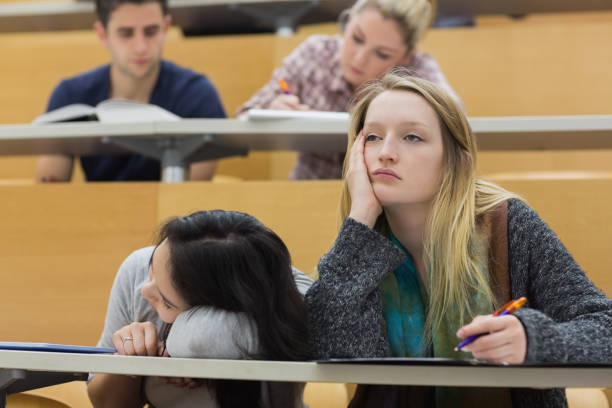
\includegraphics[width=.7\textwidth]{images/bored_student} % Replace with your image
        %\caption{Picture 3}
    \end{subfigure}
    
\end{figure}
	
\end{frame}

\begin{frame}{Why Active Learning?}
    \begin{figure}
        \centering
        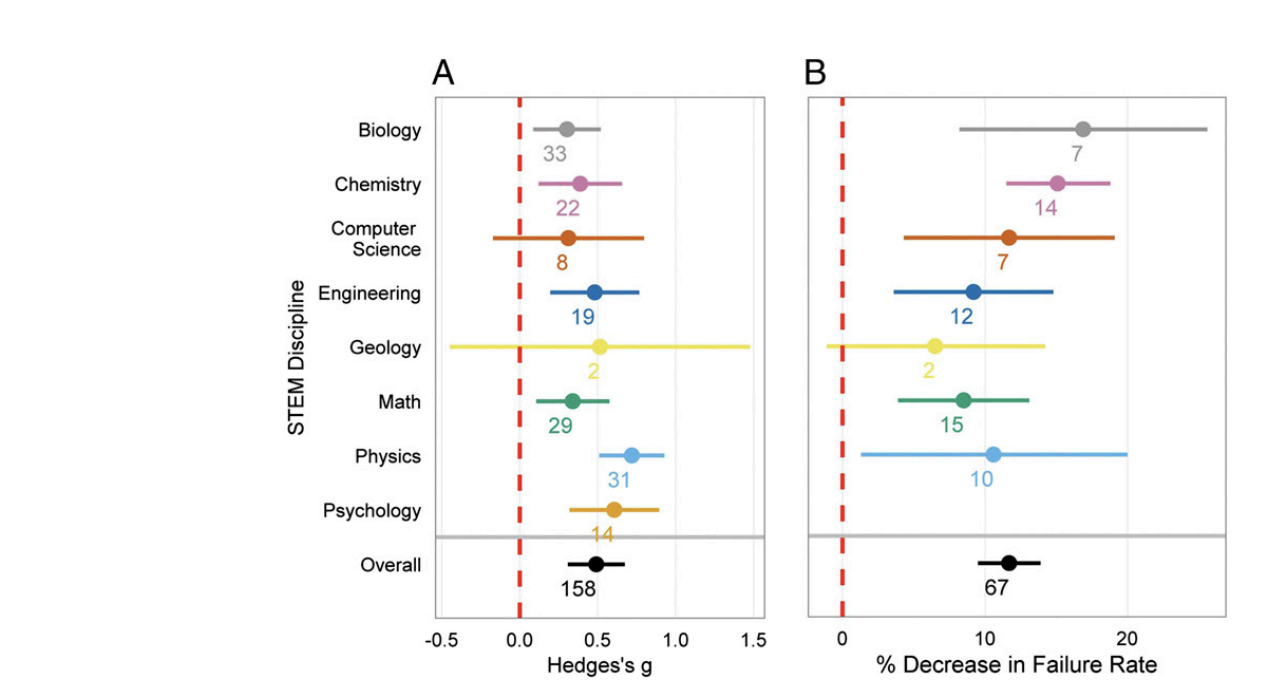
\includegraphics[width=.7\textwidth]{images/active_learning} 
    \end{figure}
	\citebottom{\hfill Freeman et al. (2014). \textit{Proceedings of the National Academy of Sciences}. \hfill }
\end{frame}

\begin{frame}{Virtues of developing mathematical reasoning}

\begin{itemize}
\item Literally makes you smarter (GRE scores).
\item Enhances study of \textit{any} domain -- not only computer science, but also cybersecurity, sociology, etc. 
\item Enhances performance at work -- often, math gets the job done better.
\item \$\$\$
\end{itemize}

\end{frame}



\begin{frame}{Virtues of developing mathematical reasoning}
    \begin{figure}
        \centering
        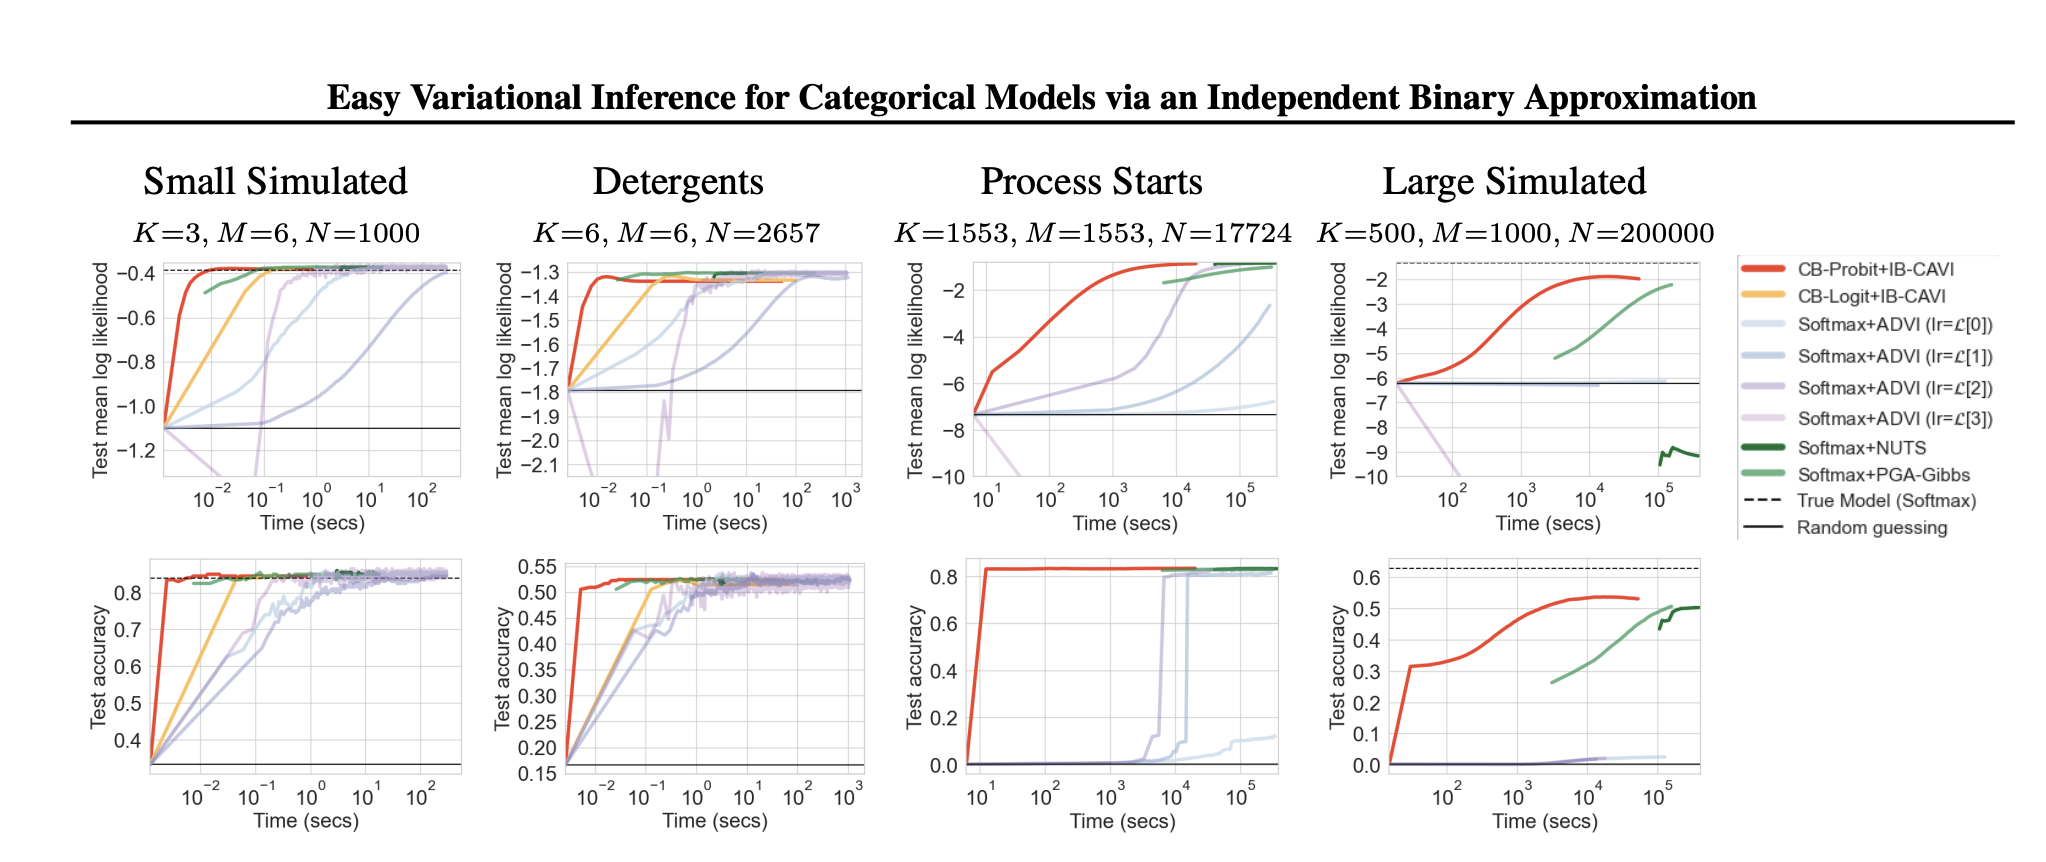
\includegraphics[width=.9\textwidth]{images/icml} 
    \end{figure}
   \citebottom{\hfill Wojnowicz et al. (2022). \textit{International Conference of Machine Learning (ICML)}. \hfill }
	
\end{frame}

\begin{frame}{Don't like math?}

\begin{itemize}
	\item Be open-minded!  Don't stereotype yourself.  % Tell story of how a Floridian learned to love Florida
	\item We're starting from scratch. (No calculus!)
	\item Stay on track by doing daily assignments.
	\item Use resources (office hours, tutoring, classmates, etc.)
	\item \textit{Growth mindset}: Anyone can improve from where they are.   
	\item \textit{Culture of confusion}: It's great to be wrong! That's how we learn. 
	\item Contact me if you're struggling.
\end{itemize}

\end{frame}


\begin{frame}{Discrete math: Example application}


Find subtle DNA copy number alterations to support \textbf{early cancer detection}.

\centering 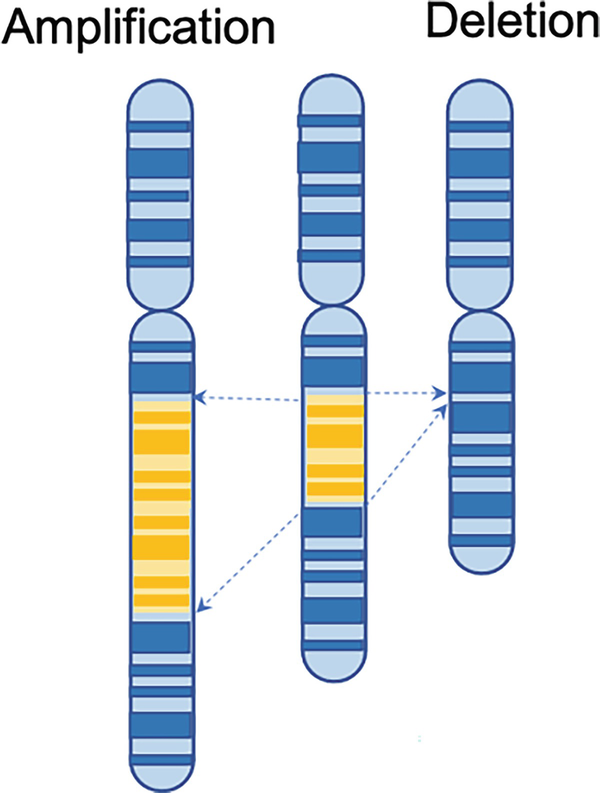
\includegraphics[width=.2\textwidth]{images/amplification_deletion} 

\citebottom{Image from: Nabavi \& Zare (2022).}

\end{frame}


\begin{frame}
\begin{columns}[T,onlytextwidth]
    \begin{column}{0.4\textwidth}
        \centering
        \vspace{1in}
        \Large How to detect changepoints within heavy noise?
     \end{column}
    \begin{column}{0.6\textwidth}	
	 \begin{center}
	  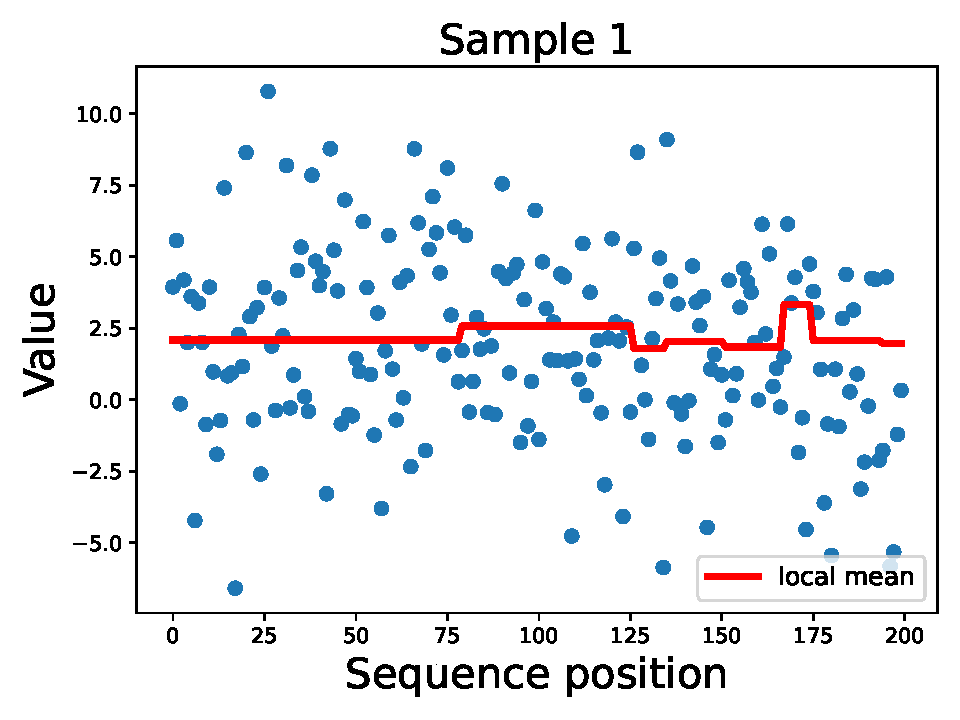
\includegraphics[width=0.5\linewidth]{images/sample_0} \\
	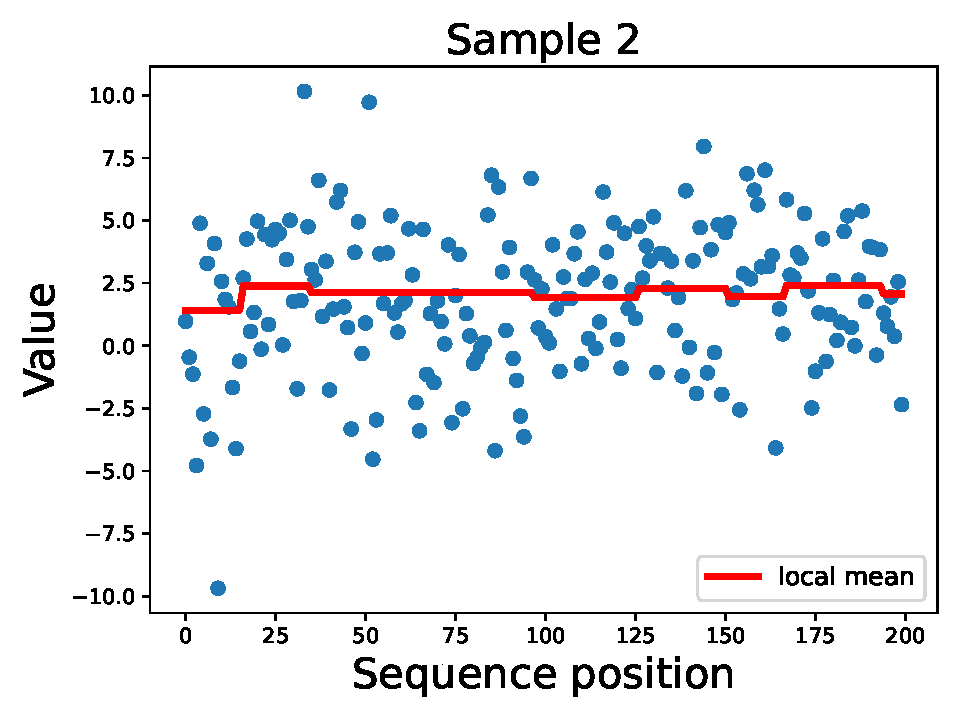
\includegraphics[width=0.5\linewidth]{images/sample_1}
	\end{center}
    \end{column}
\end{columns}

\end{frame}


\begin{frame}

\large \centering
The solution to this problem uses almost every content area we're covering in this course

\vfill 
\begin{itemize}
	\item Discrete probability 
	\item Counting
	\item Complexity (Big-O notation)
	\item Recursions
	\item Graph theory
	\item Proof techniques
\end{itemize}
\end{frame}

\end{document}
%relevant pallendrome: i prefer pi 

\input{sections/counting}

\input{sections/set-and-selection}

\input{sections/add-sub-principle}

\input{sections/inclusion-exclusion}

%\input{sections/multisets-repetition}

\input{sections/pigeonhole}

\input{sections/induction}

\input{sections/recurrence}

\input{sections/probability}

%\input{sections/binomial} %% didn't cover binom coeffs this semester

\input{sections/number-theory}


\input{sections/graph theory_ prev}



\end{document}